\documentclass{article}
\usepackage[utf8]{inputenc}
\setcounter{secnumdepth}{0}
\usepackage{graphicx}

\title{Reporte Técnico para Proyecto de Simulación e Inteligencia Artifical}

\begin{document}
\begin{titlepage}
    \centering
{\bfseries\Huge Reporte Técnico para Proyecto de Simulación e Inteligencia Artificial \par}
\vspace{2cm}
{\bfseries\Large Propuesta de modelo de movilidad humana en una ciudad mediante automotores}
\vspace{2cm}

\end{titlepage}

\section{Introducción}
El estudio de la movilidad humana, centrado en un área o ciudad determinada resulta de gran utilidad en muchos campos como la planificación urbana, la ingeniería e, incluso, la epidemiología.
El presente proyecto presenta una propuesta de modelación de movilidad humana, solo considerando movilidad mediante transporte automotor y con la aplicación de los conocimientos adquiridos en las asignaturas Simulación e Inteligencia Artificial. 

\newpage

\section{Aspectos Generales}
Para concretar el objetivo del presente proyecto, se optó por realizar una Simulación basada en Agentes. 

\subsection{Descripción de Agentes y Medio Ambiente definidos}

Un Agente es un Sistema Computacional situado dentro de un medio ambiente dentro del cual es capaz de realizar acciones para lograr sus obejtivos. Los agentes, tienen un conjunto de estados y reglas de comportamiento que lo definen. 

En el caso que se estudia, los agentes son una representación de las personas, que interactuan con el medio ambiente, en este caso la ciudad con todas sus características. 

El ambiente definido es un ambiente accesible, esto implica que el agente puede tener la información del mismo actualizada. Una persona, sabe datos de la ciudad como: los posibles lugares a los que puede desplazarse, qué transportes puede escoger para llegar a su destino, qué transportes se encuentran en su ubicación (se toma la ubicación como una Parada) e incluso qué tan lejos se encuentra un transporte determinado de su ubicación actual. El conocimiento del agente sobre el medio, le permite tomar decisiones en función de sus necesidades. Esto se explicará con más detalle próximamente.
Además es Dinámico, muchos de los cambios del ambiente son externos a la voluntad del agente. Los autobuses recorren la ciudad y siguen una ruta determinada, tienen una capacidad específica, etc.
El comportamiento del agente, no se limita solo al instante en el que está, sino valora factores como la llegada futura de transporte que le sirvan de mejor alternativa. Ejemplo: una persona A ha decidido ir hasta el Punto P. A sabe cuál es el mejor camino para llegar a P y conoce además el transporte que quiere tomar para ello. Sin embargo, puede darse el caso de que el transporte esperado llegue y A no sea capaz de montar en él. En estos casos, A deberá evaluar sus opciones, buscar otro transporte para llegar a su objetivo o mantenerse en espera del mismo. Se definen entonces agentes Reactivos, debido a que son capaces, como se explicó previamente, de percibir el estado del ambiente y tomar decisiones basadas en el mismo. Además, el agente tiene objetivos marcados y es capaz de tomar decisiones para llegar a él. Si se retoma el ejemplo del Agente A, A decide que quiere ir a P, si A ha visitado P con anterioridad, A recuerda la ruta que consideró mejor en aquel momento, y procede a decidir como seguirla. En caso de que el destino sea nuevo para A, entonces A determinará que ruta debe seguir y luego, el transporte que escoger.

\subsection{Agentes Implementados}
Se han definido dos tipos de Agentes principales que, en realidad uno es una extensión de otro. 
Primero, se define 'Person' como representación general de una persona. Cada persona tiene un identificador (en este caso se define de manera simple, puesto que no es influyente a la hora del análisis de la movilidad, más allá de que lo identifique). Una persona tiene un domicilio, lugar desde donde comienza la Simulación y al que cada día regresa en algún punto. Para esto último se definieron unos valores de preferencia de retorno al hogar, que varía según la persona y definen un intervalo donde la persona decide retornar a la casa y hacer estancia en ella. Se ha definido un atributo presupuesto, debido a que las personas con un presupuesto alto, es posible que prefieran tomar otro tipo de transporte diferente a un autobus (en este caso se pensó en Gazellas y este caso particular se explicará más adelante). 

Además de todo lo anterior mencionado, se definen otros aspectos que resultaron útiles a la hora de definir un comportamiento. Una persona sabe cuál es su ubicación actual, así como el lugar al que quiere ir (o en el que quiere estar). Como se mencionó en el apartado anterior, una vez una persona visita un lugar, o "averigua" cual es la mejor forma de llegar, en futuras ocasiones es capaz de recordar esa información sin necesidad de volver a calcularla. Por ello, se define una especie de memoria donde dado un punto de partida y un punto de destino, el agente recuerda la mejor ruta para llegar. 

El agente tiene estados que describen su situación actual. En este caso, una persona puede estar esperando una guagua, en camino a algún destino, o tal vez haciendo estancia en algún punto del mapa. Estos estados influyen en la toma de decisiones de las personas, decisiones que están definidas por acciones. Las acciones pueden ser moverse a algún destino deseado, regresar a casa o hacer estancia en el lugar actual.

Otro de los aspectos importantes a destacar son las observaciones. Como se ha mencionado, el agente puede analizar su ambiente y en base a su análisis tomar decisiones o cambiar las que había tomado previamente. Estas observaciones del ambiente son los estados de las paradas de autobuses, los autobuses que se encuentran en la parada actual, entre otras.

El otro tipo de agente que se ha definido es 'Busy Person', cuya diferencia más marcada con 'Person' es la existencia de un lugar de interés, en el que deben estar dentro de un horario determinado. La idea era reflejar una especie de rutina, ejemplo trabajadores o estudiantes que van de forma regular a un mismo lugar. Este agente tiene un cambio en su comportamiento y radica en que se encontrará, o tomará decisiones que lo lleven a ello, dentro del horario marcado en el lugar de interés.

\subsection{Medio Ambiente Implementado}
Para la implementación del Medio Ambiente, se diseñó 'Enviroment'. Resulta la clase principal con la que los agentes tienen interacción. El Medio Ambiente lo constituye el mapa de la ciudad, representado en forma de Grafo Dirigido Ponderado, donde un nodo es una Parada de Autobus y, por tanto, un posible lugar destino. Las paradas de autobus, contienen los tipos de autobuses que se detienen en ellas, así como una cola organizada de las personas que están esperandolo. Como solo se tiene en cuenta la movilidad mediante automotor, entonces la parada de autobus abarca un poco más en su concepto, pues alberga a aquellas personas que están "en zona", es decir, no están esperando un autobus ni ningún otro transporte, se ha denominado a ello como "people round". Tanto las personas que están en espera, como las que no pero se encuentran en la parada, cuentan a la hora de contabilizar las personas en un punto específico.

Los medios de transporte son una parte fundamental del proyecto. En general, se define una clase 'Transportation' que los representa. Un medio de transporte tiene un tipo, un identificador y la ruta que sigue. Para hacerlo un poco más ajustado a la realidad, los medios de transporte tienen una capacidad de personas que pueden llegar, esto significa que no siempre la persona que esté esperando X medio de transporte, será capaz de tomarlo. Los medios de transporte conocen la ubicación en la que se encuentran y siguen su ruta determinada, de manera independiente a los deseos de cualquier agente. 

Una consideración que se ha tomado es el análisis único de autobuses, aunque se deja una implementación de Gazellas, no se llega a definir las rutas para ellas en los ejemplos. 

\subsection{Estrategias para el desarrollo de la Simulación}

Para el desarrollo de la Simulación se define la clase $Simulation$ que contiene a los agentes, el medio, eventos, los datos para crear el mapa de ruta y los medios de transporte.

La función $simulate$ es la función que dirige el flujo de la simulación. Se apoya en otras funciones como: $initialize$, $run$ y $finalize$.

Primero se inicializa la Simulación. En este proceso, se crea el grafo que representará el mapa de las rutas, en base a la información que se carga y que se encuentra almacenada en un archivo .json, lo que facilita que sea sencillo cambiar a un nuevo mapa de rutas. De la misma manera, se crean los medios de transporte, con sus respectivas rutas, y se ubican en alguno de los puntos por los que pasan.

La función $run$ crea una instancia de $Enviroment$ y comienza las iteraciones de la simulación (cantidad que es previamente definida).

Dentro de las iteraciones, se recorren los diferentes puntos del mapa y se sigue la siguiente estrategia: los agentes analizan el entorno y toman una decisión, primero los que no se encuentran esperando por un transporte, luego se da seguimiento al movimiento de los medios de transporte. Al llegar a una parada, se determina qué personas dejan el vehículo y quiénes lo abordan. Por último los agentes que se han quedado esperando por un vehículo anaizan el ambiente y toman una decisión. 

La función $finalize$ cierra la simulación creando un Reporte de los movimientos, los autobuses más concurridos, las zonas de mayor interés, entre otros. Esto lo realiza gracia a los eventos que se van creando a lo largo de la simulación y con el apoyo de una clase definida llamada $Reporter$. 

Se fijan una cantidad de agentes y se crean de manera aleatoria en cuanto a su tipo, preferencia de horario, dirección de su hogar, etc. 
\section{Distribución del Proyecto}
En este apartado se detallará la distribución y organización del proyecto, así como de las clases y funciones más importantes y determinantes.

\subsection{Organzación}
\begin{itemize}
    \item En la carpeta 'agents' se encunetra la implementación de los Agentes, con sus funciones correspondientes.
    \item En la carpeta 'data' se encuentran los datos con los que se está trabajando actualmente: las rutas definidas de los autobuses y los propios autobuses.
    \item En la carpeta 'enviroment' se encuentran todas las implementaciones correspondientes al medio.
    \item En la carpeta 'extra classes' se encuentran las definiciones de los medios de transporte, grafo, nodos y paradas de autobus.
    \item En la carpeta 'pln' se encuentra la implementación de la clase $Reporter$ y todo el trabajo con la construcción del reporte final.
    \item En la carpeta 'simulation' se encuentra la implementación de la clase $Simulation$.
    \item En la carpeta 'src' se encuentran métodos auxiliares y la implementación del algoritmo de búsqueda.
    \item En la carpetta 'test' se encuentran los diferentes archivos de prueba que han servido para diferentes partes del proyecto y el archivo 'test simulation' es donde debe ejecutarse la simulación.
\end{itemize}



\subsection{Detalles de implementación}
\subsubsection{Agentes}
La lógica correspondiente a los agentes se centra en dos clases principales: $'Person'$ y $'Busy\_Person'$. 

Como ya se ha mencionado la clase $'Person'$ representa a una persona y se definieron atributos y métodos para simular su comportamiento. 
\\

Atributos:
\begin{itemize}
    \item $id$: EL identificador de la persona.
    \item $home\_dir$: Representa la dirección de residencia de la persona. (El identificador del nodo donde se encuentra).
    \item $budget$: Representa el presupuesto de la persona. (Pensado para la posibilidad de coger transporte alternativo a los autobuses).
    \item $curfew\_start$ y $curfew_end$: Representan el horario de inicio y de final de la preferencia de retornar al hogar. (Se asume que una persona en algún punto del día querrá retornar al hogar y descansar).
    \item $visited\_dir$: Representa los intervalos ya recorridos, y la ruta que el agente en su momento guardó en su memoria como la más óptima.
    \item $current\_location$: Es la ubicación actual del agente.
    \item $desired\_destiny$: Representa el lugar al que el agente desea ir.
    \item $states$: Representa los posibles estados en los que se puede encontrar el agente. 
    \item $current\_state$: Estado actual del agente.
    \item $actions$: Posibles acciones que puede tomar un agente.
    
    Además se definen unos atributos de observación, que representan lo que percibe el agente del medio, en esa instancia de tiempo.
\end{itemize}

Funciones Definidas:

\begin{itemize}
    \item $analize$: Se ocupa de percibir el ambiente y actualizar los valores necesarios de las observaciones del agente.
    \item $decide$: Permite al agente decidir su próxima acción. Para ello se tiene en cuenta detalles como: la instancia de tiempo, el estado del agente, el lugar destino del agente y algunas observaciones del ambiente.
    \item $evaluate\_decision$: Es la función que permite al agente valorar si debe cambiar una decisión previamente tomada, tiene en cuenta el estado del ambiente y los propios objetivos del agente.
    \item $move$: Función que maneja el movimiento hacia algún destino del agente. Como el agente guarda los puntos que visita y su respectiva ruta, primero se comprueba si ya conoce la ruta, si no es el caso, la busca con ayuda de la función $a\_star$.
    \item $choose\_transportation$: Función que escoge, según la ruta que se desea seguir, que transporte (o transportes) es necesario seleccionar. 
    \item $add\_visited\_dir$: Función que agrega la nueva ruta calculada a las rutas ya conocidas.
    
    Se han listado las funciones fundamentales para el funcionamiento del agente pero además se defienieron otras auxiliares que sirven de apoyo a las ya mencionadas.
\end{itemize}

En el caso de la clase $'Busy\_Person'$ se agregan algunos nuevos atributos y se realiza una modificación en la función $decide$.
\\

Atributos Agregados:
\begin{itemize}
    \item $interest\_place$: Representa la dirección del lugar donde el agente va con regularidad (escuela, trabajo, etc).
    \item $start\_time$ y $end\_time$: Representan el inicio y final, respectivamente, de la jornada de rutina. (Horario laboral, horario de clases, etc)
\end{itemize}

Todas las funciones se comportan igual que en el caso anterior, con la excepción de $decide$ que tiene en cuenta el horario de la rutina. 

\subsubsection{Ambiente}
Para la implementación del Ambiente se implementó una clase llamada $Enviroment$.
\\

Atributos:

\begin{itemize}
    \item $bus\_states$: Representa la red con todas las paradas de autobus, en este caso representada con un Grafo Dirigido.
    \item $buses$: Representan todos los autobuses que existen en el ambiente.
    \item $time$: Representa el tiempo de la simulación.
\end{itemize}

\subsubsection{Medios de Transporte}
Para el diseño de los medios de transporte se implementó la clase $Transportation$ y se definieron dos clases hijas: $Bus$ y $Gazelle$.
\\

Atributos:
\begin{itemize}
    \item $id$: Representa un identificador único para el medio de transporte,
    \item $name$: Representa la clase de medio de transporte. (Para un autobus puede ser P1 o P2, en el caso de una Gazella podría ser Ruta 19 o Ruta 14).
    \item $route$: Es la ruta (secuencia de paradas) que sigue el transporte.
    \item $capacity$: Capacidad máxima del medio de transporte. (En el caso de los autobuses debe ser mayor que las gazellas).
    \item $num\_passengers$: Cantidad de pasajeros que lleva el medio de transporte. 
    \item $is\_full$: Indicador de si el medio de transporte ha llegado a su capacidad máxima.
    \item $location$: Ubicación actual del medio de transporte.
\end{itemize}

\subsubsection{Reporter}
La clase $Reporter$ es la encargada de generar el reporte final de lo acontecido en la Simulación. 

En este proyecto se optó por utilizar la API de Gemini de Google para construir el reporte. A lo largo de la Simulación se fueron definiendo eventos, acerca de los datos de interés en la Simulación. Dichos eventos, son los datos que se le proporcionan al modelo y con el que se construye el reporte. 

Esto permite sacar conclusiones como: qué transporte ha sido el más utilizado, qué zonas son las más concurridas o con mayor interés entre los agentes, entre otros aspectos que pudieran resultar útiles al estudio de la Movilidad Humana.

\subsubsection{Otras Implementaciones}
Otras implementaciones de interés son:
\begin{itemize}
    \item $Graph$, $Node$, $Bus\_Stop$: Se realizó un implementación de Grafo Dirigido Ponderado, con sus Nodos. La clase $Bus\_Stop$ hereda de $Node$ y representa una parada de autobus. Contiene la lista de autobuses que pasan por ella, así como las colas para cada una de esos autobuses.
    \item $a\_Star$: Función donde se ha implementado el Algoritmo A* utilizado para encontrar la ruta a seguir, tomando en cuenta un nodo origen y un nodo destino determinados. La heurística escogida ha sido por Distancia Euclidiana, sin embargo, el algoritmo implementado puede usar cualquier otra heurística que se implemente.
\end{itemize}

\section{Ejemplos}

Estructura de los autobuses con los que se estarán trabajando en los ejemplos.

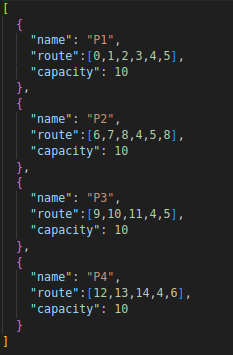
\includegraphics{buses.png}
\newpage
Estructura de mapa de rutas

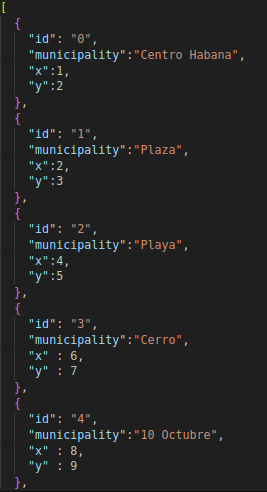
\includegraphics{m1.png}
\newline
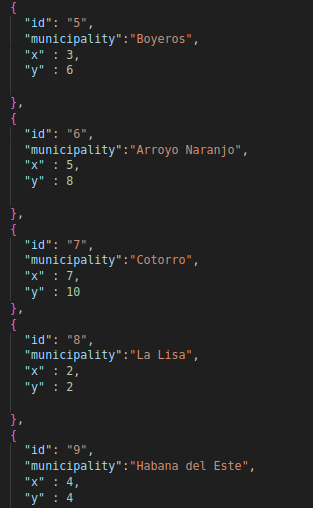
\includegraphics{m2.png}
\newline
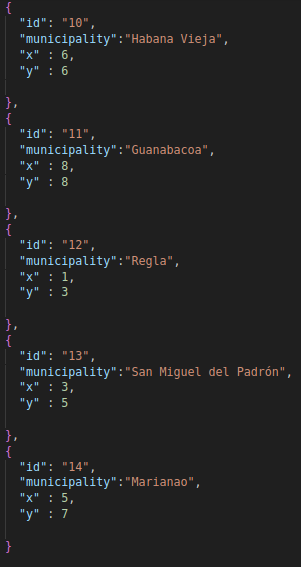
\includegraphics{m3.png}

\newpage

\subsection{Reportes obtenidos con los diferentes ejemplos: }

 

Con 2 agentes y 10 iteraciones

**Lugares Más Concurridos por las Personas**

* Parada de buses de Cerro (4 personas)
* Parada de buses de Boyeros (3 personas)

**Buses Más Utilizados**

* Bus P3 (2 personas)

Con 2 agentes y 10 iteraciones

**Paradas de buses más concurridas:**

A lo largo del período de tiempo, la parada de buses de Cerro fue consistentemente la más concurrida, con una persona presente en todas las horas.

**Buses más utilizados:**

Los buses P1 fueron los más utilizados, con una persona a bordo en las horas 5, 6, 7, 8 y 9.


Con 8 agentes y 10 iteraciones
A lo largo del día, se observaron cambios significativos en el número de personas en las paradas de buses y en el uso de los mismos. Las paradas y buses más concurridos fueron:

**Paradas de Buses Más Concurridas:**

* **Regla:** 7 personas a las 7 horas, 9 personas a las 9 horas
* **Playa:** 6 personas a las 7 horas, 7 personas a las 8 horas
* **Marianao:** 7 personas a las 9 horas
* **Plaza:** 5 personas a las 5 horas

**Buses Más Utilizados:**

* **Bus P4:** 10 personas a las 8 horas, 10 personas a las 9 horas
* **Bus P5:** 5 personas a las 5 horas, 10 personas a las 9 horas

**Patrón de Uso:**

Los datos muestran un aumento gradual en el número de personas en las paradas de buses desde las 0 horas hasta las 9 horas. La concurrencia alcanzó su punto máximo entre las 7 y las 9 horas, con una disminución posterior.

El uso de los buses también aumentó durante las horas pico de la mañana, con los buses P4 y P5 siendo los más populares. La disminución en el número de personas en las paradas de buses después de las 9 horas coincide con una menor demanda de transporte público durante las horas de la mañana.


Con 6 agentes y 10 iteraciones

**Paradas de buses más concurridas a lo largo del tiempo**

Las paradas de buses de Centro Habana y Habana Vieja fueron consistentemente las más concurridas a lo largo del día, con un promedio de 1 a 3 personas presentes en cada evento de monitoreo.

**Buses más utilizados**

Ninguno de los buses monitoreados tuvo un número significativo de pasajeros durante el período observado.

**Resumen de actividad**

* El número de personas en las paradas de buses se mantuvo relativamente constante durante la noche (0-7 horas), con un ligero aumento entre las 8 y las 9 horas.
* La actividad de los buses fue baja en general, con una ausencia total de pasajeros en todos los buses monitoreados.
* Los datos sugieren que el tráfico de pasajeros en transporte público era mínimo durante el período de monitoreo.

Con 6 agentes y 10 iteraciones

Los datos recopilados a lo largo de varias horas revelan patrones interesantes de movimiento y uso del transporte público en La Habana.

**Paradas de buses más concurridas:**

* La parada de buses de La Lisa fue la más concurrida, con 2 personas a las 6 y 7 horas.
* La parada de buses de Cerro estuvo concurrida de manera constante, con 1 persona presente en la mayoría de los intervalos de tiempo.
* Otras paradas con presencia regular de personas fueron Playa, La Lisa, San Miguel del Padrón y Marianao.

**Buses más utilizados:**

* El bus P3 fue el más utilizado, con 3 personas a bordo a las 8 y 9 horas.
* El bus P2 también tuvo un uso moderado, con 1 persona a bordo en múltiples intervalos de tiempo.

**Tendencias generales:**

* La actividad en las paradas de buses y el uso de buses fue mínimo durante las primeras horas de la mañana (0-5 horas).
* El movimiento comenzó a aumentar alrededor de las 6 horas, alcanzando su punto máximo alrededor de las 8-9 horas.
* Después de las 9 horas, la actividad disminuyó gradualmente.
* Las paradas de buses de las zonas periféricas (por ejemplo, La Lisa, San Miguel del Padrón) mostraron un mayor uso por la mañana.
* Los buses P3 y P2 fueron populares entre los viajeros en las horas pico.

 Con 8 agentes y 10 iteraciones

A lo largo de un periodo de nueve horas, se registraron patrones de movimiento de pasajeros y uso de buses en varias paradas de la ciudad.

En general, la parada de buses de Playa tuvo la mayor cantidad de pasajeros durante todo el periodo, con una presencia constante de al menos una persona. Otras paradas con un flujo constante de pasajeros fueron Habana del Este, Guanabacoa y Regla.

Los buses P1 y P5 fueron los más utilizados, con un número significativo de pasajeros a partir de las 7 de la mañana. Los buses P2, P3 y P4 tuvieron un uso relativamente bajo en comparación con los P1 y P5.

**Detalles por Hora:**

* **0:00 horas:** Playa, Cerro, Habana del Este, Guanabacoa y Regla tuvieron una sola persona cada uno.
* **1:00 a 6:00 horas:** El patrón permaneció sin cambios, con paradas similares experimentando una baja afluencia de pasajeros.
* **7:00 horas:** La parada de buses de Plaza comenzó a mostrar actividad, con una persona esperando el bus.
* **8:00 horas:** El número de pasajeros aumentó en Habana del Este, con tres personas esperando el bus.
* **9:00 horas:** El flujo de pasajeros se mantuvo estable, con cambios mínimos en las paradas más concurridas.

La información recopilada proporciona información sobre los patrones de movimiento de pasajeros a lo largo del día, lo que puede ayudar a los planificadores de transporte a optimizar los servicios de transporte público en la ciudad.

8 agentes y 24 iteraciones

**Paradas de buses más concurridas a lo largo del tiempo:**

* La parada de buses de Playa fue consistentemente la más concurrida a lo largo de todo el día.
* También fueron notables las siguientes paradas:
    * Habana Vieja
    * Habana del Este
    * San Miguel del Padrón
    * Marianao

**Buses más utilizados a lo largo del tiempo:**

* El bus P3 fue el más utilizado durante la mayor parte del día, con un máximo de 5 pasajeros a las 16:00.
* El bus P2 también tuvo un uso significativo, con 1 pasajero durante muchas horas.
* Los buses P1, P4 y P5 se usaron con menos frecuencia, con 1 pasajero cada uno en momentos específicos.

16 y 24

**Paradas de buses más concurridas a lo largo del tiempo:**

* La paradas de buses más concurridas fueron:
    * La Lisa: 4 personas
    * Boyeros: 2 personas
    * Arroya Naranjo: 2 personas
    * Cerro: 2 personas
    * Playa: 1 persona
    * Habana del Este: 1 persona
    * Plaza: 1 persona
    * Centro Habana: 1 persona
    * Cotorro: 1 persona
    * Habana Vieja: 1 persona
    * Guanabacoa: 1 persona
    * Marianao: 1 persona
    * Regla: 2 personas
    * San Miguel del Padrón: 0 personas
    * 10 de Octubre: 0 personas

**Buses más utilizados a lo largo del tiempo:**

* Los buses más utilizados fueron:
    * P5: 2 personas
    * P4: 1 personas
    * P3: 2 personas
    * P2: 2 personas
    * P1: 4 personas


50 y 24

**Puntos de mayor afluencia de personas:**

* Plaza (103 personas)
* Playa (84 personas)
* Cerro (70 personas)
* 10 de Octubre (65 personas)

**Buses más utilizados:**

* P1 (105 personas)
* P2 (94 personas)
* P3 (122 personas)
* P4 (98 personas)
* P5 (83 personas)

50 y 24

Un estudio reciente ha revelado patrones interesantes de afluencia y uso de autobuses en las zonas más concurridas de la ciudad. El estudio, que abarcó un período de 24 horas, recopiló datos sobre el número de personas en las paradas de autobús y los autobuses en varios lugares de la ciudad.

**Lugares más concurridos**

A lo largo del día, las paradas de autobús más concurridas fueron:

* Centro Habana
* Habana Vieja
* Guanabacoa
* San Miguel del Padrón
* La Lisa

**Horarios de mayor concurrencia**

Las paradas de autobús experimentaron el mayor número de personas durante las horas pico de la mañana (6-8am) y tarde (5-7pm).

**Autobuses más utilizados**

Los autobuses que más se utilizaron durante el período de estudio fueron:

* Bus P4 (10 personas en promedio)
* Bus P5 (6 personas en promedio)
* Bus P3 (6 personas en promedio)

50 y 24
**Resumen de los lugares más concurridos por las personas a lo largo del tiempo:**

* **Centro Habana:** Altamente concurrido durante todo el día, con un pico entre las 13:00 y las 18:00 horas.
* **Plaza:** Concurrencia constante durante todo el día, con un ligero aumento entre las 14:00 y las 20:00 horas.
* **Playa:** Concurrido principalmente durante las horas pico (07:00-09:00 y 17:00-19:00 horas).
* **La Lisa:** Concurrencia alta durante todo el día, con un ligero descenso entre las 12:00 y las 15:00 horas.
* **Habana del Este:** Concurrencia constante durante todo el día, con un aumento notable entre las 17:00 y las 21:00 horas.

**Resumen de los buses más utilizados:**

* **P1:** Altamente utilizado durante todo el día, con un pico entre las 07:00 y las 09:00 horas y entre las 17:00 y las 20:00 horas.
* **P2:** Uso moderado durante todo el día, con un ligero aumento entre las 13:00 y las 17:00 horas.
* **P3:** Uso intenso durante todo el día, con un pico entre las 13:00 y las 18:00 horas.
* **P4:** Uso alto entre las 07:00 y las 12:00 horas y entre las 16:00 y las 20:00 horas.
* **P5:** Uso significativo entre las 07:00 y las 12:00 horas y entre las 16:00 y las 21:00 horas.



\section{Propuestas de Mejoría}
Como propuestas de mejorías, el equipo plantea los siguientes puntos:
\begin{itemize}
    \item En el proyecto original en el que se basó la idea del presente, se recomendaba obtener los mapas, paradas de autobus y rutas de dos aplicaciones específicas. Al principio se consideró esa vía pero, por motivos de requerimientos de los equipos y de espacio, no se pudo hacer de esa manera. El equipo considera que sería provechoso poder usar esos mapas y rutas mucho más cercanos a la realidad que los definidos de ejemplo. 
    \item Inicialmente se pensó en la idea de Gazellas, transportes con menos capacidad, más comodidad y más caros, sin embargo al final no se implementaron los mapas y sus rutas, a pesar de haber definido su clase y facilidades para ello. Sería interesante incluir las Gazellas como alternativa de medio de transporte, pues variaría más el comportamiento de aquellos agentes con presupuesto alto. 
    \item Se podrían definir otros tipos de Agentes, con características más específicas que variaran más el rumbo de la simulación, así como otros elementos del ambiente a tener en cuenta en la toma de decisiones.
    \item Para los algoritmos de búsqueda de rutas, y decisiones de los agentes, se sigue una estrategia definida en cada caso, se deja la posibilidad de definir otras heurísticas o estrategias en ambos casos e incluso, hacer que dependa de la preferencia del propio agente.
    \item Se recomiendan implementar mejoras en la organización del proyecto, así como en la optimización de alguno de los métodos implementados.
\end{itemize}

\section{Conclusiones}
Se ha desarrollado un proyecto que es capaz de Simular la Movilidad Humana teniendo en cuenta solo vehículos dado un mapa y un conjunto de medios de transporte específico. Para ello fueron necesarios integrar conocimientos obtenidos a lo largo del curso en las asignaturas de Inteligencia Artificial y Simulación. 

La teoría acerca de Agentes y Medio, permitió tener ideas más claras acerca de cómo abordar el problema y cómo diseñar las respectivas estructuras para representarlos.

Para encontrar la mejor ruta, dada una estrategia específica se recurrió al Algoritmo A*, con una heurística sencilla pero con posibilidad de implementar cualquier otra en dependencia del objetivo deseado.

Los Agentes pueden recurrir a sus experiencias previas, para escoger las rutas y son capaces de reaccionar ante los cambios del medio, evaluando sus opciones y tomando una decisión en base a sus objetivos.

Se presenta un Reporte de lo acontecido y datos de interés, en cuanto a movilidad humana, mediante Procesamiento de Lenguaje Natural, y la definición de eventos.

Se plantearon las recomendaciones y las mejoras que el equipo cree pertinentes o que podrían resultar enriquecedoras para el proyecto.
\end{document}
